%%%%%%%%%%%%%%%%%%%%%%%%%%%%%%%%%%%%%%%%%
% Beamer Presentation -- ICPSR Causal Inference
% Day 8 (June 24, 2026): A model of an observational study; matching for comparability and effective sample size
% Source: Leavitt and Miratrix (2026), Sections 2.1-2.2.3
%%%%%%%%%%%%%%%%%%%%%%%%%%%%%%%%%%%%%%%%%

%------------------------------------------------------------------------------------------------
% PACKAGES AND THEMES
%------------------------------------------------------------------------------------------------

\documentclass[table, xcolor = {dvipsnames}, 9pt]{beamer}
\usepackage{tikz}
\usetikzlibrary{calc}
\usetikzlibrary{positioning}
\usetikzlibrary{arrows.meta}
\usetikzlibrary{external}
\mode<presentation> {
\usetheme{metropolis}
\usecolortheme{seagull}
\usefonttheme{professionalfonts}
}

\usepackage{graphicx} % Allows including images
\usepackage{booktabs} % Allows the use of \toprule, \midrule and \bottomrule in tables
\usepackage{float}
\usepackage{tikz}
\usepackage{multirow}
\usepackage{natbib}
\usepackage{hyperref}
\usepackage{diagbox}
\usepackage{makecell}
\usepackage{xparse}
\usepackage{subfig}
\usepackage{amsmath}
\usepackage{amsfonts,amsthm,amsmath,amssymb}
\usepackage{bbm}
\usepackage{bm}
\usepackage{empheq}
\usepackage{pgfplots}
\usepackage{animate}
\usepgfplotslibrary{colorbrewer}
\pgfplotsset{compat=1.17}

\newcommand\mybox[2][]{\tikz[overlay]\node[fill=lightgray,inner sep=2pt, anchor=text, rectangle, rounded corners=1mm,#1] {#2};\phantom{#2}}
\hypersetup{unicode=true,
            bookmarksnumbered=true,
            bookmarksopen=true,
            bookmarksopenlevel=2,
            breaklinks=false,
            pdfborder={0 0 1},
            hypertexnames=false,
            pdfstartview={XYZ null null 1}}
\usepackage{xcolor}
% R code listing style (matches the course's R-code slides)
\usepackage{listings}
\definecolor{codegreen}{rgb}{0,0.6,0}
\definecolor{codegray}{rgb}{0.5,0.5,0.5}
\definecolor{codepurple}{rgb}{0.58,0,0.82}
\definecolor{backcolour}{rgb}{0.95,0.95,0.92}
\lstdefinestyle{Rstyle}{
    language=R,
    backgroundcolor=\color{backcolour},
    commentstyle=\color{codegreen},
    keywordstyle=\color{magenta},
    stringstyle=\color{codepurple},
    basicstyle=\ttfamily\footnotesize,
    breakatwhitespace=false,
    breaklines=true,
    keepspaces=true,
    showspaces=false,
    showstringspaces=false,
    showtabs=false,
    tabsize=2
}
\newcommand\myheading[1]{%
  \par\bigskip
  {\Large\bfseries#1}\par\smallskip}
\newcommand\given[1][]{\:#1\vert\:}
\theoremstyle{plain}
\newtheorem{thm}{Theorem}
\newtheorem{prop}{Proposition\thisthmnumber}
\newtheorem{lem}{Lemma\thisthmnumber}
\newtheorem{cor}{Corollary}
\newtheorem{defin}{Definition}
\newtheorem{algo}{Algorithm}
\newcommand*\diff{\mathop{}\!\mathrm{d}}
\newcommand*\Diff[1]{\mathop{}\!\mathrm{d^#1}}
\newcommand{\bh}[1]{{\color{blue}{#1}}}
\newcommand{\mh}[1]{{\color{magenta}{#1}}}
\newcommand{\thisthmnumber}{}
\newcommand{\tikzmark}[1]{\tikz[baseline,remember picture] \coordinate (#1) {};}
\newcommand*{\QEDA}{\hfill\ensuremath{\blacksquare}}%
\newcommand*{\QEDB}{\hfill\ensuremath{\square}}%
\newcommand{\abs}[1]{\left\lvert #1 \right\rvert}
\DeclareMathOperator{\E}{\rm{E}}
\DeclareMathOperator{\R}{\mathbb{R}}
\DeclareMathOperator{\N}{\mathbb{N}}
\DeclareMathOperator{\Var}{\rm{Var}}
\DeclareMathOperator{\Cov}{\rm{Cov}}
\DeclareMathOperator{\Supp}{\rm{Supp}}
\DeclareMathOperator{\e}{\rm{e}}
\DeclareMathOperator{\F}{\mathcal{F}}
\DeclareMathOperator{\Z}{\mathcal{Z}}
\DeclareMathOperator{\logit}{\rm{logit}}
\DeclareMathOperator{\indep}{{\perp\!\!\!\perp}}
\DeclareMathOperator{\rank}{rank}
\DeclareMathOperator*{\argmin}{arg\,min}
\DeclareMathOperator*{\argmax}{arg\,max}

%------------------------------------------------------------------------
% TITLE PAGE -- Day 8 (June 24, 2026)
% Source: Leavitt and Miratrix (2026), Sections 2.1-2.2.3
%-----------------------------------------------------------------------
\pagestyle{empty}
\title[A model of an observational study]{A Model of an Observational Study: Matching for Comparability and Effective Sample Size}

\author{Thomas Leavitt}
\institute[]
{
\medskip
\textit{}
}
\date{June 24, 2026}

\begin{document}

\begin{frame}
\titlepage
\end{frame}

%------------------------------------------------------------------------
\begin{frame}[t]{Where we are: from experiments to observation}
\vfill
\begin{itemize} \vfill
\item Experiments: random assignment gave \mh{known} treatment probabilities \vfill
\item Known chances $\Rightarrow$ unbiased estimates, tests, CIs \vfill
\item Now: observational data --- we do \emph{not} control assignment \vfill
\item We observe units \emph{after} treatment was assigned \vfill
\item Treatment probabilities are \mh{unknown}, possibly depending on covariates \vfill
\item Today: \mh{recreate} a completely block-randomized experiment via matching \vfill
\item Today: understanding \mh{comparability} and \mh{effective sample size} \vfill
\item Tomorrow: \mh{construct} the optimal matches, then assess them \vfill
\end{itemize} \vfill
\end{frame}
%------------------------------------------------------------------------
\section{A model of an observational study}

\begin{frame}[t]{Assignment on the basis of a covariate}
\vfill
\begin{itemize} \vfill
\item Treatment is \emph{not} randomized --- we only observe who was treated ($Z_i = 1$) \vfill
\item Each unit gets an \mh{independent} coin --- its chance a function of $x_i$ \vfill
\item[]
\begin{equation*}
\Pr\!\left(Z_i = 1\right) = e(x_i), \qquad 0 < e(x_i) < 1
\end{equation*} \vfill
\item $e(\cdot)$ is an \mh{arbitrary} function; $x_i$ is unit $i$'s fixed covariate value \vfill
\item \emph{Same} $x \Rightarrow$ same chance $e(x)$; different $x \Rightarrow$ different chance \vfill
\item We need \emph{not} know $e(\cdot)$ --- only that units sharing $x$ share $e(x)$ \vfill
\item Rubin's \mh{assignment on the basis of a covariate} \citep{rubin1977} \vfill
\end{itemize} \vfill
\end{frame}
%------------------------------------------------------------------------
\begin{frame}[t]{Step 1: the probability of one assignment}
\vfill
\begin{itemize} \vfill
\item Within stratum $S$: the $n_S$ units share one $p = e(x)$ \vfill
\item Coins are \mh{independent} $\Rightarrow$ an assignment $\bm{z}_S$ has probability (a product): \vfill
\item[]
\begin{equation*}
p(\bm{z}_S) = \prod_{i \in S} p^{\,z_i}(1-p)^{\,1 - z_i} = p^{\sum_i z_i}(1-p)^{\sum_i (1 - z_i)} = p^{\,m_S}(1-p)^{\,n_S - m_S}
\end{equation*} \vfill
\item $m_S = \sum_{i \in S} z_i$ is the number treated; exponents \mh{add} across the product \vfill
\item Only the \mh{count} $m_S$ enters --- not which units (same $p$ across $S$) \vfill
\end{itemize} \vfill
\end{frame}
%------------------------------------------------------------------------
\begin{frame}[t]{Step 2: condition on the count $\Rightarrow$ uniform}
\vfill
\begin{itemize} \vfill
\item \mh{Conditional probability}, in general: $\Pr(A \mid B) = \dfrac{\Pr(A \cap B)}{\Pr(B)}$ \vfill
\item $A = \{\bm{Z}_S = \bm{z}_S\}$, and $B$ fixes the treated count at $m_S$ \vfill 
\item[] Since $\bm{z}_S$ has $m_S$ treated, $A \subseteq B$ \vfill
\item So $\Pr(A \cap B) = \Pr(A) = p(\bm{z}_S)$ \vfill
\item[] denominator sums over the $\binom{n_S}{m_S}$ such $\bm{z}_S$ \vfill
\item[]
\begin{equation*}
p(\bm{z}_S \mid m_S) = \frac{p^{m_S}(1-p)^{n_S-m_S}}{\binom{n_S}{m_S}\, p^{m_S}(1-p)^{n_S-m_S}} = \binom{n_S}{m_S}^{-1}
\end{equation*} \vfill
\item The $p$ factors \mh{cancel}: uniform $=$ \mh{complete random assignment} within $x$ \vfill
\end{itemize} \vfill
\end{frame}
%------------------------------------------------------------------------
\begin{frame}[fragile]{A numeric look: conditioning yields a uniform}
\begin{lstlisting}[style=Rstyle, basicstyle=\ttfamily\tiny, frame=single]
# plogis(u) = 1 / (1 + exp(-u)): inverse-logit, maps any real u to (0, 1)
e <- function(x) plogis(-1 + 0.8 * x)    # Pr(Z_i = 1) = e(x_i): a function of x
x_S <- 2
n_S <- 4
p   <- e(x = x_S)                        # 4 units share x = 2, so one common p

all_z  <- as.matrix(expand.grid(rep(x = list(c(0, 1)), times = n_S)))
m_of_z <- rowSums(all_z)                 # number treated in each assignment z
# Pr(Z = z): a PRODUCT because coins are independent; one p because same x within S
pr_z   <- p^m_of_z * (1 - p)^(n_S - m_of_z)

m       <- 2                             # condition on m_S = 2 treated
keep    <- m_of_z == m
pr_cond <- pr_z[keep] / sum(pr_z[keep])  # renormalize: act as-if CRA within S
round(pr_cond, 4)                        # all equal: 0.1667 ...
1 / choose(n = n_S, k = m)               # 1/6 = 0.1667  (p has cancelled)
\end{lstlisting}
\begin{itemize} \vfill
\item Each assignment with $m_S$ treated gets the \mh{same} conditional probability \vfill
\item A different $x$ gives a different $p$, the \emph{same} uniform --- $p$ \mh{cancels} \vfill
\end{itemize}
\end{frame}
%------------------------------------------------------------------------
\begin{frame}[t]{What conditioning on $x$ buys us}
\vfill
\begin{itemize} \vfill
\item Within each $x$-group, fixing the treated count $\Rightarrow$ \mh{uniform} assignment \vfill
\item We do \emph{not} need the probabilities $e(x)$ \vfill
\item Only that they are the \mh{same} for units with the same $x$ \vfill
\item That \mh{assumption} is the precise sense of as-if randomization \vfill
\end{itemize} \vfill
\end{frame}
%------------------------------------------------------------------------
\begin{frame}[t]{From a covariate to a matched-set covariate}
\vfill
\begin{itemize} \vfill
\item Exact conditioning is easy for a single, discrete $x$ \vfill
\item But $\bm{x}$ is usually multivariate, often continuous $\to$ exact matches are rare \vfill
\item \mh{Matching} builds sets $s = 1, \dots, S$ of units with similar $\bm{x}$ \vfill
\item $b_i \in \{1, \dots, S\}$, the \mh{matched-set label}, now plays the role of $x$ \vfill
\item Condition on $b_i$: compare treated vs.\ control \emph{only within} each set \vfill
\item \mh{Hope}: within a set, treatment \emph{probabilities} are equal \vfill
\begin{itemize} \vfill
\item[$\ast$] $b_i$ is $\bm{Z}$-dependent, not a fixed baseline --- set aside here \\ \citep{pashleyetal2021,pimentelhuang2024,pimentelyu2024} \vfill
\end{itemize} \vfill
\item We check the hope indirectly, via balance (tomorrow's last act) \vfill
\end{itemize} \vfill
\end{frame}
%------------------------------------------------------------------------
\section{Where matching fits}

\begin{frame}[t]{Design before analysis \citep{leavittmiratrix2026}}
\vfill
\begin{itemize} \vfill
\item Units already wound up treated or control, via an \mh{unknown} mechanism \vfill
\item Matching is a \mh{design} choice --- \emph{after} that, but \emph{before} we see outcomes \vfill
\item The full pipeline has three stages: \vfill
\begin{itemize} \vfill
\item \textbf{1.} build and evaluate matched sets \vfill
\item \textbf{2.} infer causal effects under as-if randomization \vfill
\item \textbf{3.} assess sensitivity to departures from it \vfill
\end{itemize} \vfill
\item Today lives \emph{entirely} in \mh{Stage 1} (the shaded block, next) \vfill
\end{itemize} \vfill
\end{frame}
%------------------------------------------------------------------------
\begin{frame}{The matching pipeline \citep{leavittmiratrix2026}}
\vfill
\begin{figure}
\centering
\includegraphics[width=\textwidth,height=0.77\textheight,keepaspectratio]{figures/matching_pipeline_flowchart.pdf}
\caption*{\scriptsize Flow diagram of the design-based matching pipeline \citep{leavittmiratrix2026}}
\end{figure}
\vfill
\end{frame}
%------------------------------------------------------------------------
\begin{frame}[t]{Stage 1 is five questions --- a two-day roadmap}
\vfill
\begin{itemize} \vfill
\item \textbf{Today:} \vfill
\begin{itemize} \vfill
\item How do I \mh{measure similarity} on my covariates? \vfill
\item including the \mh{estimated propensity score} \vfill
\item How do I ensure \mh{comparability}? \vfill
\item How do I improve \mh{effective sample size}? \vfill
\end{itemize} \vfill
\item \textbf{Tomorrow:} \vfill
\begin{itemize} \vfill
\item How do I actually \mh{form} the matches? \vfill
\item How do I decide whether to \mh{move ahead} with the matched design? \vfill
\end{itemize} \vfill
\end{itemize} \vfill
\end{frame}
%------------------------------------------------------------------------
\section{The running example}

\begin{frame}{Motivating example: UN peacekeeping}
\vfill
\begin{figure}
\centering
\includegraphics[width=0.78\linewidth]{figures/UN_Peacekeepers.png}
\caption*{\scriptsize \textbf{UN Mission in Liberia.} Nigerian peacekeepers serving with UNMIL.\\ \textit{UN Photo/Albert Gonz\'{a}lez Farran, Monrovia, Liberia, 2018.}}
\end{figure}
\vfill
\end{frame}
%------------------------------------------------------------------------
\begin{frame}[t]{UN peacekeeping and post-conflict peace \citep{gilligansergenti2008}}
\vfill
\begin{itemize} \vfill
\item \textbf{Unit}: a \mh{post-conflict peace episode} (peace after a civil war) \vfill
\item E.g.\ Sierra Leone, Jan 2001--Dec 2003; $87$ episodes, 1989--2003 \vfill
\item \textbf{Treatment} \texttt{UN} $=1$ if a UN mission was \mh{present}, else $0$ \vfill
\item[] $19$ treated, $68$ control \vfill
\item \textbf{Outcome} \texttt{ldur}: log days of peace until conflict (or censoring) \vfill
\item The question: does UN presence \mh{prolong} post-conflict peace? \vfill
\end{itemize} \vfill
\end{frame}
%------------------------------------------------------------------------
\begin{frame}{``UN missions are not randomly assigned''}
\begin{figure}
\centering
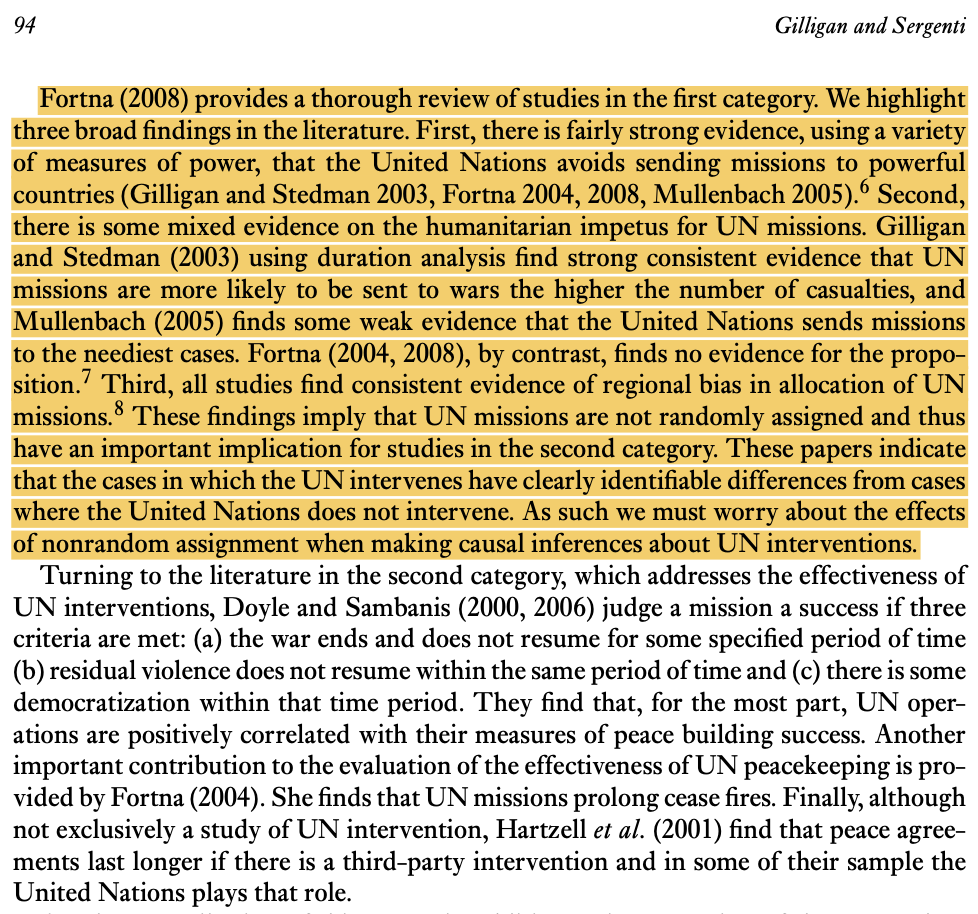
\includegraphics[width=0.66\linewidth]{figures/Gilligan_Sergenti_2008_p_94.png}
\caption*{\scriptsize \citet[][p.~94]{gilligansergenti2008} on the non-random assignment of UN interventions}
\end{figure}
\end{frame}
%------------------------------------------------------------------------
\begin{frame}[t]{The nine covariates we match on}
\vfill
\begin{itemize} \vfill
\item Pre-treatment characteristics presumed to drive UN intervention: \vfill
\begin{itemize} \vfill
\item logged war deaths (\texttt{lwdeaths}), logged previous-war duration (\texttt{lwdurat}) \vfill
\item ethnic fractionalization (\texttt{ethfrac}, $0$--$100$), logged population (\texttt{pop}) \vfill
\item logged mountainous terrain (\texttt{lmtnest}), logged military personnel (\texttt{milper}) \vfill
\item logged pre-war GDP per capita (\texttt{bwgdp}), Polity score (\texttt{bwplty2}, $-10$ to $10$) \vfill
\item \texttt{region} (E.\ Europe, Lat.\ America, Asia, S.S.\ Afr., N.\ Afr./Mid.\ East) \vfill
\end{itemize} \vfill
\item Many are also \mh{prognostic} --- a further reason to match \\ \citep{hansen2008a,salesetal2018} \vfill
\item \mh{Transformations} (logs, scales) are the authors', taken as given \vfill
\end{itemize} \vfill
\end{frame}
%------------------------------------------------------------------------
\begin{frame}[fragile]{Setup: load the data and covariates in \texttt{R}}
\begin{lstlisting}[style=Rstyle, basicstyle=\ttfamily\tiny, frame=single]
library(optmatch)   # match_on(), exactMatch(): distances and exact-match strata
library(dplyr)      # mutate() for the region dummies

data <- readRDS(url(   # 87 post-conflict peace episodes
  "https://raw.githubusercontent.com/tl2624/matching-guide/main/data/peace_pre_match.rds"))
covs <- c("lwdeaths", "lwdurat", "ethfrac", "pop", "lmtnest", "milper",
          "bwgdp", "bwplty2", "region")

# Expand the region factor into 0/1 dummies (Euclidean needs numeric covariates)
data <- data |> mutate(
  eeurop   = ifelse(region == "eeurop",   1, 0),
  lamerica = ifelse(region == "lamerica", 1, 0),
  asia     = ifelse(region == "asia",     1, 0),
  ssafrica = ifelse(region == "ssafrica", 1, 0),
  nafrme   = ifelse(region == "nafrme",   1, 0))
expanded_covs <- c(setdiff(covs, "region"),
                   "eeurop", "lamerica", "asia", "ssafrica", "nafrme")
\end{lstlisting}
\end{frame}
%------------------------------------------------------------------------
\section{How do I measure similarity on my chosen covariates?}

\begin{frame}[t]{The distance matrix}
\vfill
\begin{itemize} \vfill
\item To match, we first need a \mh{distance}: how close are any two units? \vfill
\item Record in a matrix: \textbf{rows} treated, \textbf{columns} control \vfill
\item Each cell: two units' covariates $\to$ one \mh{nonnegative} number \vfill
\item[] smaller $=$ more similar \citep{rubinwaterman2006} \vfill
\item Goal: build sets of units that are \mh{close} on this measure \vfill
\end{itemize} \vfill
\end{frame}
%------------------------------------------------------------------------
\begin{frame}[t]{Euclidean distance}
\vfill
\begin{itemize} \vfill
\item \mh{Euclidean}: square root of the sum of squared covariate differences \vfill
\item[]
\begin{equation*}
d(\bm{x}_i, \bm{x}_j) = \sqrt{\sum_{k} (x_{ik} - x_{jk})^2}
\end{equation*} \vfill
\item $\bm{x}_i$: unit $i$'s covariate vector; $x_{ik}$: its $k$th covariate \vfill
\item Categorical \texttt{region} first expanded into $0/1$ dummy indicators \vfill
\item Example: treated \mh{Liberia} vs.\ control \mh{Guinea-Bissau} $\approx 57.44$ \vfill
\end{itemize} \vfill
\end{frame}
%------------------------------------------------------------------------
\begin{frame}[fragile]{Euclidean distance: Liberia vs.\ Guinea-Bissau}
\begin{lstlisting}[style=Rstyle, basicstyle=\ttfamily\tiny, frame=single]
liberia       <- data[data$cname == "Liberia",       expanded_covs]
guinea_bissau <- data[data$cname == "Guinea-Bissau", expanded_covs]
sqrt(sum((liberia - guinea_bissau)^2))                 # 57.44
\end{lstlisting}
\vspace{-0.3em}
\scriptsize
\begin{table}[H]
\centering
\begin{tabular}{lrrr}
\toprule
Covariate & Liberia & Guinea-Bissau & Sq.\ diff. \\
\midrule
\texttt{lwdeaths} & 10.04 & 7.52 & 6.35 \\
\texttt{lwdurat} & 69.00 & 12.00 & 3249.00 \\
\texttt{ethfrac} & 82.99 & 80.38 & 6.84 \\
\texttt{pop} & 7.91 & 7.19 & 0.52 \\
\texttt{lmtnest} & 0.47 & 0.00 & 0.22 \\
\texttt{milper} & 1.61 & 1.95 & 0.11 \\
\texttt{bwgdp} & 6.02 & 5.24 & 0.61 \\
\texttt{bwplty2} & $-6.00$ & 0.00 & 36.00 \\
\texttt{region} dummies & \multicolumn{2}{c}{\footnotesize both Sub-Saharan Africa} & 0.00 \\
\midrule
\textbf{TOTAL} & & & \textbf{3299.66} \\
\bottomrule
\end{tabular}
\end{table}
\normalsize
\vspace{-0.2em}
\begin{itemize}
\item $\sqrt{3299.66} \approx \mh{57.44}$ --- \texttt{lwdurat} alone contributes $3249$ \vfill
\end{itemize}
\end{frame}
%------------------------------------------------------------------------
\begin{frame}[t]{Two problems with Euclidean distance}
\vfill
\begin{itemize} \vfill
\item \mh{Scale}: a large-scale covariate \emph{dominates} \vfill 
\item[] \texttt{lwdurat} drove most of Liberia--Guinea's $57.44$ \vfill
\item \mh{Correlation}: \texttt{pop} and \texttt{milper} largely reflect \emph{one} factor ($\approx 0.79$) \vfill
\item[] bigger countries have both more people and more soldiers \vfill
\item Euclidean adds both \emph{separately}, double-counting that factor \vfill
\item[] $\Rightarrow$ \mh{inflated} distance \vfill
\end{itemize} \vfill
\end{frame}
%------------------------------------------------------------------------
\begin{frame}[t]{Mahalanobis distance \citep{mahalanobis1936}}
\vfill
\begin{itemize} \vfill
\item Fixes \emph{both} problems at once: \vfill
\begin{itemize} \vfill
\item \mh{standardizes} each covariate onto a comparable (SD) scale \vfill
\item adjusts for \mh{correlations}, so related covariates are not double-counted \vfill
\end{itemize} \vfill
\item A \mh{statistical device}, not substantive --- transforms (logs) come \emph{first} \vfill
\end{itemize} \vfill
\end{frame}
%------------------------------------------------------------------------
\begin{frame}[fragile]{Mahalanobis distance: Liberia vs.\ Guinea-Bissau}
\begin{lstlisting}[style=Rstyle, basicstyle=\ttfamily\tiny, frame=single]
mcovs <- setdiff(covs, "region")             # 8 numeric covariates
S_inv <- solve(cov(data[, mcovs]))           # inverse covariance matrix
d     <- as.numeric(data[data$cname == "Liberia",       mcovs] -
                    data[data$cname == "Guinea-Bissau", mcovs])
sqrt(t(d) %*% S_inv %*% d)                    # 2.79
\end{lstlisting}
\vspace{-0.3em}
\scriptsize
\begin{table}[H]
\centering
\begin{tabular}{lrrr}
\toprule
Covariate & Liberia & Guinea-Bissau & Contribution \\
\midrule
\texttt{lwdeaths} & 10.04 & 7.52 & 0.53 \\
\texttt{lwdurat} & 69.00 & 12.00 & 0.08 \\
\texttt{ethfrac} & 82.99 & 80.38 & 0.06 \\
\texttt{pop} & 7.91 & 7.19 & 1.75 \\
\texttt{lmtnest} & 0.47 & 0.00 & 0.19 \\
\texttt{milper} & 1.61 & 1.95 & 0.94 \\
\texttt{bwgdp} & 6.02 & 5.24 & 1.87 \\
\texttt{bwplty2} & $-6.00$ & 0.00 & 2.36 \\
\midrule
\textbf{TOTAL} & & & \textbf{7.79} \\
\bottomrule
\end{tabular}
\end{table}
\normalsize
\vspace{-0.2em}
\begin{itemize}
\item $\sqrt{7.79} \approx \mh{2.79}$ --- big \mh{variance} $\Rightarrow$ small contribution \vfill
\item \texttt{lwdurat}'s huge variance shrinks its gap: $3249 \to 0.08$ \vfill
\end{itemize}
\end{frame}
%------------------------------------------------------------------------
\begin{frame}[fragile]{The distance matrix in practice}
\begin{lstlisting}[style=Rstyle, basicstyle=\ttfamily\tiny, frame=single]
cov_fmla     <- reformulate(termlabels = covs, response = "UN")  # region as factor
dist_mat_mah <- match_on(x = cov_fmla, data = data,
                         standardization.scale = NULL, method = "mahalanobis")
\end{lstlisting}
\begin{itemize} \vfill
\item One \mh{Mahalanobis} distance per treated--control pair: \vfill
\end{itemize}
\footnotesize
\begin{table}[H]
\centering
\begin{tabular}{lrrrr}
\toprule
Treated $\downarrow$ / Control $\rightarrow$ & Niger & Guinea & Togo & C.\ Afr.\ Rep. \\
\midrule
Sierra Leone & 2.14 & 2.23 & 2.65 & 2.91 \\
Zaire & 4.30 & 3.73 & 4.63 & 4.14 \\
Rwanda & 4.84 & 3.96 & 4.96 & 4.47 \\
Mozambique & 3.58 & 3.69 & 3.65 & 4.12 \\
Namibia & 5.31 & 4.47 & 4.96 & 4.24 \\
\bottomrule
\end{tabular}
\end{table}
\normalsize
\begin{itemize}
\item Lower $=$ more similar; Sierra Leone--Niger ($2.14$) is the closest shown \vfill
\end{itemize}
\end{frame}
%------------------------------------------------------------------------
\subsection{The propensity score}

\begin{frame}[t]{The curse of dimensionality}
\vfill
\begin{itemize} \vfill
\item With \mh{many} covariates, hard to find units similar on \emph{all} of them \vfill
\item \mh{Propensity score} $\lambda(\bm{x}_i) = \Pr(Z_i = 1 \mid \bm{x}_i)$: \vfill 
\item[] Treatment probability given the \emph{observed} covariates $\bm{x}_i$ \vfill
\item This is the model's $e$, now a function of the \emph{whole} vector $\bm{x}_i$ \vfill
\item Collapses all covariates into \mh{one} number \vfill
\item[] $\lambda$ is unobserved $\Rightarrow$ we match on its \emph{estimate} \vfill
\end{itemize} \vfill
\end{frame}
%------------------------------------------------------------------------
\begin{frame}[t]{Estimating the propensity score}
\vfill
\begin{itemize} \vfill
\item We do not know $\lambda$; \mh{estimate} it by logistic regression $\to \hat{\lambda}(\bm{x}_i)$ \vfill
\item $\hat{\lambda} = $ \mh{inverse-logit} of the estimated linear index $\bm{\hat{\beta}}^{\top}\bm{x}_i$, in $(0,1)$: \vfill
\item[]
\begin{equation*}
\logit^{-1}(u) = \frac{1}{1 + e^{-u}} \in (0,1), \qquad \hat{\lambda}(\bm{x}_i) = \logit^{-1}\!\left(\bm{\hat{\beta}}^{\top}\bm{x}_i\right)
\end{equation*} \vfill
\item Read $\hat{\lambda}$ or its estimated linear index as one useful \mh{1-D score} (monotone transforms) \vfill
\item[] \emph{not} necessarily unbiased or consistent estimator of $\lambda$ \vfill
\item $\bm{\hat{\beta}}$: \mh{estimated} coefficients from the fitted logistic regression \vfill
\end{itemize} \vfill
\end{frame}
%------------------------------------------------------------------------
\begin{frame}[t]{What the estimated linear index does}
\vfill
\begin{itemize} \vfill
\item The fit makes the index \mh{high for treated}, low for control \vfill
\item Little treated/control \mh{overlap} $\to$ predictive $\to$ \mh{large} coefficient \vfill
\item Much overlap $\to$ weakly predictive $\to$ small coefficient \vfill
\item Net: covariates weighted by how strongly they predict \emph{treatment} \vfill
\end{itemize} \vfill
\end{frame}
%------------------------------------------------------------------------
\begin{frame}[fragile]{Fitting the propensity score in \texttt{R}}
\begin{lstlisting}[style=Rstyle, basicstyle=\ttfamily\tiny, frame=single]
# Exclude region: some regions (near-)perfectly predict treatment (separation)
psm_cov_fmla <- reformulate(termlabels = setdiff(x = covs, y = "region"),
                            response = "UN")
psm <- glm(formula = psm_cov_fmla, family = binomial(link = "logit"), data = data)

# Estimated linear index = linear predictor = logit of the estimated PS
lin_cov_inds <- psm$linear.predictors
p_scores     <- psm$fitted.values
all.equal(lin_cov_inds, log(p_scores / (1 - p_scores)))   # TRUE
\end{lstlisting}
\begin{itemize} \vfill
\item \texttt{lin\_cov\_inds}: each unit's \mh{estimated} linear index $\bm{\hat{\beta}}^{\top}\bm{x}_i$ \vfill
\item \texttt{p\_scores}: the \mh{estimated} propensity scores $\hat{\lambda}(\bm{x}_i)$ \vfill
\item Excluding \texttt{region} avoids (near-)perfect prediction (separation) \vfill
\end{itemize}
\end{frame}
%------------------------------------------------------------------------
\begin{frame}{Why similar indices? Namibia vs.\ Burundi}
\vfill
\begin{itemize} \vfill
\item They \emph{differ} on \texttt{lwdurat}, \texttt{ethfrac} --- but those have \mh{small} coefficients \vfill
\item They are \emph{similar} on \texttt{milper} --- which has a \mh{large} coefficient \vfill
\item[]
\footnotesize
\begin{table}[H]
\centering
\begin{tabular}{lrrr}
\toprule
 & \texttt{lwdurat} & \texttt{ethfrac} & \texttt{milper} \\
\midrule
Namibia (treated) & 269 & 67.7 & 2.30 \\
Burundi (control) & 98 & 3.55 & 2.56 \\
estimated coefficient & $-0.01$ & $0.00$ & $-0.92$ \\
\bottomrule
\end{tabular}
\end{table}
\normalsize
\vfill
\item Big raw gaps $\times$ \mh{tiny} coefficients $\Rightarrow$ contributions are small \vfill
\item Indices end up close ($0.01$ vs.\ $0.51$) on a range $-7.5$ to $2.2$ \vfill
\end{itemize}
\end{frame}
%------------------------------------------------------------------------
\begin{frame}{Reading overlap on the linear covariate index}
\begin{itemize}
\item Boxplots of the index by group: where do treated and control \mh{overlap}? \vfill
\item Treated cluster near $\mathbf{0}$; many controls sit far \mh{below} \vfill
\item[]
\begin{figure}[H]
\includegraphics[width=0.64\linewidth]{figures/lin_cov_index_boxplot.pdf}
\end{figure}
\item[] \footnotesize Index $0 \Leftrightarrow \hat{\lambda} = 0.5$ --- where treated and control \mh{overlap} most. \normalsize
\end{itemize}
\end{frame}
%------------------------------------------------------------------------
\begin{frame}[fragile]{Euclidean distance in the estimated propensity score}
\begin{lstlisting}[style=Rstyle, basicstyle=\ttfamily\tiny, frame=single]
data$p_score <- p_scores
liberia <- data[data$cname == "Liberia",       "p_score"]
guinea  <- data[data$cname == "Guinea-Bissau", "p_score"]
sqrt((liberia - guinea)^2)                     # 0.57
\end{lstlisting}
\vspace{-0.2em}
\footnotesize
\begin{table}[H]
\centering
\begin{tabular}{lr}
\toprule
Country & Estimated propensity score \\
\midrule
Liberia & 0.74 \\
Guinea-Bissau & 0.17 \\
\midrule
\textbf{Absolute difference} & \textbf{0.57} \\
\bottomrule
\end{tabular}
\end{table}
\normalsize
\begin{itemize} \vfill
\item Distance on \emph{one} scalar replaces distance on all $8$ covariates \vfill
\item Liberia far more ``treatment-like'' ($0.74$) than Guinea-Bissau ($0.17$) \vfill
\end{itemize}
\end{frame}
%------------------------------------------------------------------------
\section{How can I apply rules for matches to ensure comparability?}

\begin{frame}[t]{Two ways to forbid bad matches}
\vfill
\begin{itemize} \vfill
\item Improve balance by \emph{excluding} matches that are ``too dissimilar'': \vfill
\item \textbf{Exact matching}: require identical values on a (categorical) covariate \vfill
\item \textbf{Caliper}: a maximum allowable distance; farther pairs are forbidden \vfill
\item Illustration with two simple constraints: \vfill
\begin{itemize} \vfill
\item same \mh{region} only (exact match) \vfill
\item Polity scores within \mh{2} points (caliper) \vfill
\end{itemize} \vfill
\end{itemize} \vfill
\end{frame}
%------------------------------------------------------------------------
\begin{frame}[fragile]{Calipers as $\infty$ distances}
\begin{lstlisting}[style=Rstyle, basicstyle=\ttfamily\tiny, frame=single]
# Exact match on region: 0 within a region, Inf across regions
em_region <- exactMatch(x = UN ~ region, data = data)

# Caliper of 2 on Polity (bwplty2): Inf when units differ by more than 2 points
euc_dist_polity_cal_2 <- match_on(x = UN ~ bwplty2, caliper = 2, data = data,
                                  standardization.scale = NULL, method = "euclidean")

# Combine constraints by ADDING distance objects (Inf if EITHER is violated)
overall_dist_mat <- em_region + euc_dist_polity_cal_2
\end{lstlisting}
\begin{itemize} \vfill
\item \texttt{optmatch} minimizes the total within-set distance \vfill
\item A distance of $\infty$ (\texttt{Inf}) makes a pair \mh{impossible} to match \vfill
\item \mh{Adding} distance objects: a pair is barred if \emph{either} is $\infty$ \vfill
\item Rule of thumb: PS caliper $\le 0.2$ SD of the logit \\ \citep{cochranrubin1973} \vfill
\end{itemize}
\end{frame}
%------------------------------------------------------------------------
\begin{frame}{Calipers rule out matches in the distance matrix}
\vfill
\begin{itemize} \vfill
\item \textbf{Example}: forbid any match with Mahalanobis distance $> 3$ \vfill
\item A violated caliper sets the cell to $\infty$ --- an \mh{impossible} match \vfill
\item[] \vfill
\footnotesize
\begin{table}[H]
\centering
\begin{tabular}{lrrrr}
\toprule
Treated $\downarrow$ / Control $\rightarrow$ & Niger & Guinea & Togo & C.\ Afr.\ Rep. \\
\midrule
Sierra Leone & 2.14 & 2.23 & 2.65 & 2.91 \\
Zaire & $\infty$ & $\infty$ & $\infty$ & $\infty$ \\
Rwanda & $\infty$ & $\infty$ & $\infty$ & $\infty$ \\
Mozambique & $\infty$ & $\infty$ & $\infty$ & $\infty$ \\
Namibia & $\infty$ & $\infty$ & $\infty$ & $\infty$ \\
\bottomrule
\end{tabular}
\end{table}
\normalsize
\vfill
\item Only treated Sierra Leone stays matchable here; other treated \mh{ruled out} \vfill
\end{itemize} \vfill
\end{frame}
%------------------------------------------------------------------------
\section{How can I apply rules for matches to improve effective sample size?}

\begin{frame}[t]{Size is not just a head count}
\vfill
\begin{itemize} \vfill
\item Design goal: \mh{maximize} effective sample size at acceptable balance \vfill
\item We care about the matched study's size --- not the raw total \vfill
\item \mh{Effective sample size}: a sum of within-set harmonic means \vfill
\begin{equation*}
\sum_{s=1}^S \left[\left(m_s^{-1} + (n_s - m_s)^{-1}\right)/2\right]^{-1}
\end{equation*} \vfill
\item $m_s$ treated, $n_s - m_s$ control; depends on the \mh{arrangement} \vfill
\item Intuition: a set's harmonic mean $=$ its \mh{equivalent number of matched pairs} \vfill
\end{itemize} \vfill
\end{frame}
%------------------------------------------------------------------------
\begin{frame}[t]{Why arrangement matters: $4$ units}
\vfill
\begin{itemize} \vfill
\item \textbf{Two matched pairs}: $\left[(1^{-1}+1^{-1})/2\right]^{-1}\!\times 2 = 2$ \vfill
\item \textbf{One set}, $1$ treated $+$ $3$ control: $\left[(1^{-1}+3^{-1})/2\right]^{-1} = 1.5$ \vfill
\item Two pairs give two comparisons --- more information \vfill
\item Harmonic mean is largest when the counts are \mh{equal} \vfill
\item Anticipates inference: \vfill 
\item[] \mh{Minimizes} Diff-in-Means variance under \mh{constant} effects \\ \citep{hansenbowers2008} \vfill
\end{itemize} \vfill
\end{frame}
%------------------------------------------------------------------------
\begin{frame}[t]{Levers on effective sample size}
\vfill
\begin{itemize} \vfill
\item \mh{Relax calipers} (Polity $2 \to 3$): in this case, more controls $\to$ more \mh{lopsided}  \vfill
\item Lopsided sets typically add little $\to$ ESS rises only \emph{slightly} \vfill
\item \mh{Ratio constraints}: bound the control-to-treated ratio per set \vfill
\item In practice: iterate, checking balance \emph{and} size \citep{hansensales2015} \vfill
\end{itemize} \vfill
\end{frame}
%------------------------------------------------------------------------
\begin{frame}[t]{Ratio constraints: \texttt{min.controls}, \texttt{max.controls}}
\vfill
\begin{itemize} \vfill
\item In \texttt{fullmatch()}, bound the control-to-treated ratio per set \vfill
\item E.g.\ $\geq 1$ control per $2$ treated: \texttt{min.controls = 0.5} \vfill
\item E.g., $\leq 2$ controls per treated: \texttt{max.controls = 2} \vfill
\item Possible consequences: \vfill
\begin{itemize} \vfill
\item Balance can \emph{worsen} --- a control forced onto a less-similar unit \\ 
\phantom{Balance can \emph{worsen} --- } (but still within caliper) \vfill
\item Or ESS can \emph{improve} --- regrouping without hurting balance \vfill
\item Too \mh{stringent} $\Rightarrow$ units discarded $\Rightarrow$ ESS falls \vfill
\end{itemize} \vfill
\end{itemize} \vfill
\end{frame}
%------------------------------------------------------------------------
\section{Looking ahead}

\begin{frame}[t]{Recap: building blocks of a matched design}
\vfill
\begin{itemize} \vfill
\item \mh{Matching} aims to recreate a completely block-randomized experiment \vfill
\item A \mh{distance} turns two units' covariates into one similarity number \vfill
\item Euclidean $\to$ Mahalanobis $\to$ rank-based distances \vfill
\item The \mh{propensity score} collapses many covariates into one index \vfill
\item Exact matches and calipers \mh{forbid} non-comparable pairs ($\infty$ distance) \vfill
\item \mh{Effective sample size} rewards balanced sets (harmonic mean) \vfill
\item Tomorrow: \mh{construct} the optimal matches, then assess them \vfill
\end{itemize} \vfill
\end{frame}
%------------------------------------------------------------------------
\begin{frame}[allowframebreaks]
\frametitle{References}
\scriptsize
\bibliographystyle{chicago}
\bibliography{Bibliography}
\end{frame}
%------------------------------------------------------------------------
\end{document}
